
%--------------------------------------------------------------------
%--------------------------------------------------------------------
% Formato para los talleres del curso de Métodos Computacionales
% Universidad de los Andes
%--------------------------------------------------------------------
%--------------------------------------------------------------------

\documentclass[11pt,letterpaper]{exam}
\usepackage[utf8]{inputenc}
\usepackage[spanish]{babel}
\usepackage{graphicx}
\usepackage{tabularx}
\usepackage[absolute]{textpos} % Para poner una imagen en posiciones arbitrarias
\usepackage{multirow}
\usepackage{float}
\usepackage{hyperref}
\decimalpoint

\begin{document}
\begin{center}
{\Large Métodos Computacionales} \\
Taller 5 --- 2018-10\\

\end{center}


\vspace{0.3cm}

\noindent
La solución a este taller debe subirse por SICUA antes de las 5:00PM
del lunes 14 de mayo del 2018. 
Si se entrega la tarea antes del lunes 23 de abril del 2018 a las
11:59PM los ejercicios se van a calificar con el bono indicado. 
\noindent

\vspace{0.3cm}
Los archivos del c\'odigo  deben estar en un \'unico repositorio 
\verb"NombreApellido_taller5", por ejemplo si su nombre es Malena
Pichot el repositorio debe llamarse \verb"MalenaPichot_taller5". 
Al clonarlo debe crearse la carpeta \verb"MalenaPichot_taller5"
con tres carpetas: \verb"punto_1", \verb"punto_2" y \verb"punto_3"

En la implementaci\'on principal de los algoritmos solicitados la
copia y reutilizaci\'on de c\'odigo de cualquier fuente de internet
(inclu\'ido el repositorio del curso) deja la nota en cero.  

Todas las respuestas deben ser escritas en C++ y cada carpeta debe
incluir el makefile para compilar el c\'odigo, ejecutarlo y producir
la gr\'afica solicitada.

\begin{questions}




\question{\bf{Condensador de placas paralelas}}

(20 puntos) Considere un condensador de placas paralelas ubicado
en una regi\'on bidimensional del espacio, de dimensiones $L\times
L$. Las placas tienen un largo $l$ y una separaci\'on $d$ entre ellas, como se
muestra en la figura \ref{fig:gridplates}. 

\begin{figure}[H]
  \centering
  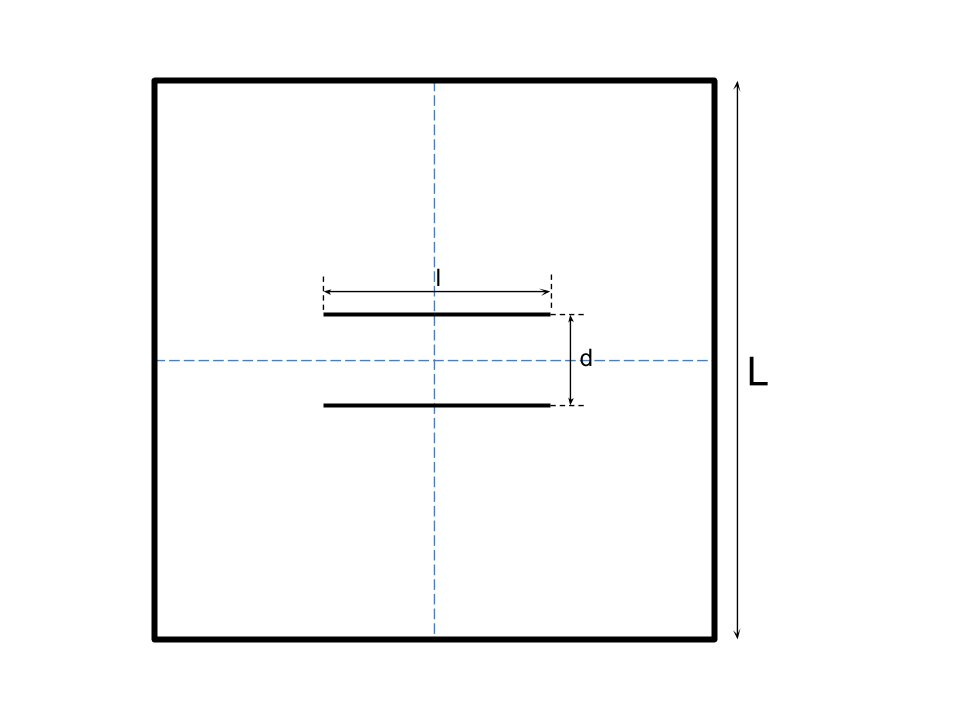
\includegraphics[width=10cm]{gridplates}
  \caption{\label{fig:gridplates} Condensador de placas paralelas.}
\end{figure}

Supongamos que existe una diferencia de potencial constante $V_0$
entre las placas (una de las placas se encuentra a $-V_0/2$ y la otra
a $V_0/2$). Adem\'as, en el borde de la regi\'on tomemos el potencial
fijo en $0$. 

El potencial el\'ectrico $V(x,y)$ en la regi\'on debe cumplir la
ecuaci\'on de Laplace 

\begin{equation}
 \nabla^2V(x,y) = \frac{\partial^2 V(x,y)}{\partial x^2} +
 \frac{\partial^2 V(x,y)}{\partial y^2}=0. 
\end{equation}

As\'i mismo el campo el\'ectrico est\'a dado por.
\begin{equation}
\mathbf{E}(x,y) = -\nabla V(x,y) = \left(-\frac{\partial V(x,y)}{\partial x}, -\frac{\partial V(x,y)}{\partial y}\right)
\end{equation}

Para calcular el potencial num\'ericamente se debe discretizar la
regi\'on como una matriz de tama\~no $L/h \times L/h$, donde $h$ es la
separaci\'on entre los puntos y utilizar el esquema de diferencias
finitas. 

Escriba un programa en C++ (\verb"placas.cpp") que encuentre el
potencial el\'ectrico con el m\'etodo de relajaci\'on usando N
iteraciones. El mismo programa debe calcular el campo el\'ectrico a
partir de la soluci\'on final del potencial.
Escriba un c\'odigo en Python \verb'grafica.py' que grafique el
potencial y el campo el\'ectrico usando \verb'imshow' y
\verb'streamplot' en una grafica llamada \verb'placas.pdf'.

Utilice $L = 5$ cm, $l = 2$ cm, $d = 1$ cm, $h = 5/512$ cm, $V_0 = 100$ V y $N = 2\times (L/h)^2$ iteraciones.
 

\question{{\bf Caos}}

(40 (45) puntos) Escriba un c\'odigo para resolver el siguiente
sistema de ecuaciones con un m\'etodo Runge-Kutta de cuarto orden.

\begin{equation}
\dot{q}_2 = p_1,
\end{equation}

\begin{equation}
\dot{q}_2 = p_2,
\end{equation}

\begin{equation}
\dot{p}_1 = -\frac{2q_1}{(4q_1^2 + \epsilon^2)^{3/2}},
\end{equation}

\begin{equation}
\dot{p}_2 = \frac{q_1 - q_2}{((q_1 - q_2)^2 + \epsilon^2/4)^{3/2}} -
\frac{q_1+q_2}{((q_1 + q_2)^2 + \epsilon^{2}/4)^{3/2}}.
\end{equation}


Tome un paso de tiempo $\Delta t=0.006$, un tiempo total de
$t=3000$, condiciones iniciales $(q_1, p_1)=(a,0)$ y $(q_2,
p_2)=(-a,0)$ con $a=1/(2\sqrt{2})$ y $\epsilon=10^-3$.


El movimiento descrito por $q_1$ es peri\'odico. Para visualizar el
comportamiento de las variables, cada vez que $q_1$ pase de ser
positivo a negativo el c\'odigo va a imprimir en pantalla los valores de $q_2$
y $p_2$.  Luego un c\'odigo de python debe preparar la gr\'afica de
$q_2$ vs. $p_2$.

El c\'odigo fuente debe llamarse \verb"caos.cpp", el ejecutable
\verb"caos.x", el script de python para hacer la gr\'afica
\verb"caos.py" y la gr\'afica final \verb"caos.pdf".



\end{questions}


Nota: Utilice esta libreria \verb"https://github.com/glennrp/libpng" para leer y escribir las
im\'agenes. 
Para la transformada de Fourier debe escribir su propia implementaci\'on.
En todos los casos el ejecutable debe poder crearse con el comando
\verb"make". 
\end{document}.
